\chapter{Récurrence}
\section*{Quelques définitions}
    \subsection*{La suite de Fibonacci}
        La suite de Fibonacci est définie de manière récurrente comme suit :
            \(
                F_0 = 0, \ F_1 = 1, \ F_{n+2} = F_{n+1} + F_n \text{ pour } n \geq 0.
            \)

        Elle commence par 0 puis 1, et chaque terme suivant est la somme des deux termes précédents :
            0, 1, 1, 2, 3, 5, \ldots
\subsection*{Les coefficients binomiaux}
    Les coefficients binomiaux sont définis à partir du symbole \(\displaystyle \binom{n}{k}\), qui représente le nombre de façons de choisir \(k\) éléments parmi \(n\) éléments, sans tenir compte de l'ordre. Ils sont donnés par la formule suivante :
    \[
        \binom{n}{k} = \frac{n!}{k!(n-k)!}, \quad \text{pour } 0 \leq k \leq n.
    \]

    Les coefficients binomiaux apparaissent naturellement dans le développement du binôme de Newton :
    \[
        (a + b)^n = \sum_{k=0}^n \binom{n}{k} a^{n-k} b^k.
    \]

\section*{Exercices (simples) sur les nombres de Fibonacci}
\begin{exercise}
    Démontrer la formule de Binet pour les nombres de Fibonacci :
    \[
        F_n = \frac{\alpha^n - \beta^n}{\sqrt{5}},\
        \text{ où } \alpha = \frac{1 + \sqrt{5}}{2} \text{ et } \beta = \frac{1 - \sqrt{5}}{2}.
    \]

    \textbf{Indication :} Utiliser la relation de récurrence \(F_{n+2} = F_{n+1} + F_n\).
\end{exercise}

\begin{exercise}
    Montrer que les nombres de Fibonacci peuvent être exprimés sous forme combinatoire :
    \[
    F_n = \binom{n-1}{0} + \binom{n-2}{1} + \binom{n-3}{2} + \cdots.
    \]
    \textbf{Indication :} Étudier les coefficients binomiaux et la relation avec la définition des \(F_n\).
\end{exercise}

\begin{exercise}
    Prouver que la somme des carrés des \(n\) premiers nombres de Fibonacci est donnée par la relation :
    \[
    \sum_{i=1}^n F_i^2 = F_n F_{n+1}.
    \]
    \textbf{Indication :} Utiliser une démonstration par récurrence pour valider cette identité.
\end{exercise}

\begin{exercise}
    Démontrer l'identité matricielle suivante pour les nombres de Fibonacci :
    \[
    \begin{pmatrix}
    1 & 1 \\
    1 & 0
    \end{pmatrix}^n =
    \begin{pmatrix}
    F_{n+1} & F_n \\
    F_n & F_{n-1}
    \end{pmatrix}.
    \]
    \textbf{Indication :} Utiliser la définition de la puissance matricielle et la relation de récurrence des nombres de Fibonacci.
\end{exercise}

\section*{Quelques exercices}
\begin{exercise} % Problème 15
    Soit \(\alpha\) un nombre réel tel que \(\alpha + \frac{1}{\alpha} \in \mathbb{Z}\).

    \begin{enumerate}
        \item Vérifiez que si \(\alpha = 2 + \sqrt{3}\), alors \(\alpha + \frac{1}{\alpha} = 4\).

        \item En supposant que, pour tout entier \(k\) tel que \(1 \leq k \leq n\), on a \(\alpha^k + \frac{1}{\alpha^k} \in \mathbb{Z}\), montrez que cela reste vrai pour \(n+1\), c'est-à-dire que \(\alpha^{n+1} + \frac{1}{\alpha^{n+1}} \in \mathbb{Z}\).

        \item Concluez que pour tout \(n \in \mathbb{N}\), \(\alpha^n + \frac{1}{\alpha^n} \in \mathbb{Z}\).
    \end{enumerate}
\end{exercise}

\begin{exercise} % Problème 16
    Le but de cet exercice est de montrer que, pour tout entier \(n \geq 1\), la somme suivante est comprise entre 1 et 2 :
    \[
    S = \frac{1}{n+1} + \frac{1}{n+2} + \cdots + \frac{1}{3n+1}.
    \]

    \begin{enumerate}
        \item Déterminer, en fonction de $n$, le nombre de termes de cette somme.
        \item Quel est le plus petit terme de cette somme ? et le plus grand ?
        \item Montrez que \(1 < S < 2\).
    \end{enumerate}
\end{exercise}

\begin{exercise}
    On veut montrer que tous les nombres de la forme \(1007, 10017, 100117, \dots\) sont divisibles par \(53\).

    \begin{enumerate}
        \item Écrivez un terme général \(a_n\) pour décrire cette suite de nombres.
        \item Quelle est la différence entre deux termes consécutifs de cette suite ?
        \item Concluez que \(a_n\) est divisible par \(53\) pour tout \(n \geq 1\).
    \end{enumerate}
\end{exercise}

\begin{exercise}
    Soient \(x_1, x_2\) les racines de l'équation \(x^2 + px - 1 = 0\), où \(p\) est un entier impair.
    On définit \(y_n = x_1^n + x_2^n\) pour tout \(n \geq 0\).
    Montrer que \(y_n\) et \(y_{n+1}\) sont des entiers premiers entre eux.

    \begin{enumerate}
        \item Calculez $y_0$, $y_1$, puis $\mathrm{pgcd}(y_0,y_1)$.
        \item Établissez la relation $y_{n+2} = -p \, y_{n+1} + y_n$.
        \item Déduire que \(\mathrm{pgcd}(y_n, y_{n+1}) = 1\) pour tout \(n \geq 0\).
    \end{enumerate}
\end{exercise}

\begin{exercise}
    On considère \(2n\) points donnés dans l'espace, et \(n^2 + 1\) segments de droite tracés entre ces points. Montrer qu'il existe au moins un ensemble de trois points qui sont reliés deux à deux par des segments de droite.

    \begin{enumerate}
        \item Expliquez pourquoi un graphe avec \(2n\) sommets et sans triangle peut avoir au maximum \(n^2\) arêtes.
            % Utilisez, si nécessaire, un graphe biparti complet pour illustrer cet argument.
        \item En déduire qu'un graphe contenant \(2n\) sommets et \(n^2 + 1\) arêtes doit nécessairement contenir au moins un triangle.
    \end{enumerate}
\end{exercise}



%%%%%%%%%%%%%%
\section*{Quelques problèmes}

\begin{problem}
Montrez que pour tout $n \in \mathbb{N}$, nous avons $f(n) = g(n)$, où
\[
f(n) = 1 - \frac{1}{2} + \frac{1}{3} - \dots + \frac{1}{2n+1} - \frac{1}{2n}, \quad g(n) = \frac{1}{n+1} + \dots + \frac{1}{2n}.
\]
\end{problem}

\begin{problem}
Montrez que $(n+1)(n+2) \cdots 2n = 2^n \cdot 1 \cdot 3 \cdot 5 \cdot \dots \cdot (2n-1)$ pour tout $n \in \mathbb{N}$.
\end{problem}

\begin{problem}
Montrez que $3^{n+1}$ divise $2^{3n} + 1$ pour tout entier $n \geq 0$.
\end{problem}
\begin{problem}
Soit $n = 2^k$. Montrez qu'il est possible de sélectionner $n$ entiers parmi $(2n-1)$ entiers de telle sorte que leur somme soit divisible par $n$.
\end{problem}

\begin{problem}
Tous les nombres de la forme $12008$, $120308$, $1203308$, $\dots$ sont divisibles par $19$.
\end{problem}

\begin{problem}
    $n$ cercles sont donnés dans le plan.
    Ils divisent le plan en plusieurs parties.
    Montrez qu'il est possible de colorier le plan avec deux couleurs de telle sorte qu'aucune partie ayant une frontière commune avec une autre ne soit coloriée de la même couleur.
    Une telle coloration est appelée une \emph{coloration propre}.
\end{problem}

\begin{problem}
%{Le Probl\`eme des Trominos}
    \begin{multicols}{2}
        \subsection*{Qu'est-ce qu'un tromino ?}
            Un \textbf{tromino} est une forme compos\'ee de trois carr\'es connect\'es par leurs c\^ot\'es.
            Dans ce probl\`eme, nous consid\'erons uniquement les trominos en forme de \textit{L}, c'est-\`a-dire trois carr\'es formant un angle droit.

        \vspace{1\baselineskip}
        \subsection*{Qu'est-ce qu'un pavage ?}
            Un \textbf{pavage} consiste \`a recouvrir enti\`erement une surface avec des formes sans chevauchement ni espace vide.
            Ici, nous cherchons \`a recouvrir une grille carr\'ee en utilisant uniquement des trominos.

        \columnbreak

        \noindent\resizebox{\linewidth}{!}{%
        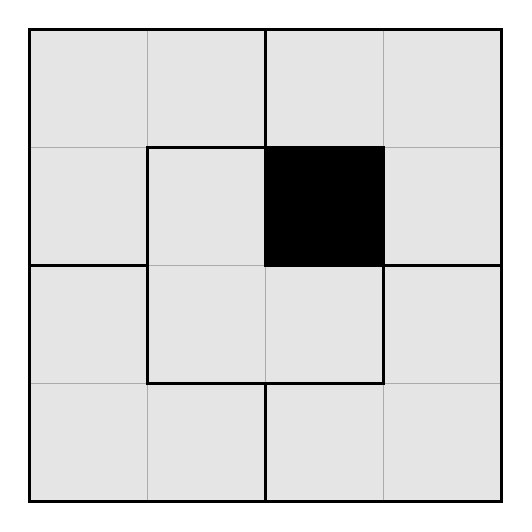
\begin{tikzpicture}[scale=1.5]
            \draw[very thick, fill=gray!20!white] (-2,0) -- (-1,0) -- (-1,1) -- (0,1) -- (0,2) -- (-2,2) -- cycle;
            \draw[very thick, fill=gray!20!white] (0,-2) -- (2,-2) -- (2,0) -- (1,0) -- (1,-1) -- (0,-1) -- cycle;
            \draw[very thick, fill=gray!20!white] (2,2) -- (2,0) -- (1,0) -- (1,1) -- (0,1) -- (0,2) -- cycle;
            \draw[very thick, fill=gray!20!white] (-2,-2) -- (-2,0) -- (-1,0) -- (-1,-1) -- (0,-1) -- (0,-2) -- cycle;
            \draw[very thick, fill=gray!20!white] (-1,-1) -- (1,-1) -- (1,0) -- (0,0) -- (0,1) -- (-1,1) -- cycle;
            \draw[opacity=.25] (-2,-2) grid (2,2);
            \draw[fill=black] (0,0) rectangle (1,1);
        \end{tikzpicture}}
    \end{multicols}

        \vspace{2\baselineskip}
        On consid\`ere une grille carr\'ee de taille $2^n \times 2^n$, o\`u $n$ est un entier positif. Un des carr\'es de cette grille est colori\'e en noir.

        \textbf{Question :} Est-il possible de recouvrir tous les autres carr\'es de la grille avec des trominos en forme de \textit{L}, sans chevauchement et sans laisser de case vide ?
\end{problem}
